\chapter{Mechanical protein unfolding via AFM}
\label{sec:methods}

In this chapter we will review the basic methods and procedures for
mechanically unfolding proteins with an atomic force microscope.  We
will discuss the working principle behind an AFM (\cref{sec:afm}) and
outline the procedure for synthesizing protein chains
(\cref{sec:polymer-synthesis}).  With the groundwork out of the way,
we will look at sample preparation (\cref{sec:sample-preparation}) and
the velocity clamp force spectroscopy procedure
(\cref{sec:procedure}).  Finally, we will give a summary of cantilever
calibration (\cref{sec:cantilever-calib:intro}) which is discussed in
more detail in \cref{sec:cantilever-calib}.

Everything discussed in this chapter, with the possible exception of
cantilever calibration, is fairly standard practice in the field of
force spectroscopy.  See \cref{sec:cantilever-calib} for the
development of the cantilever calibration theory from first principles
and references to related papers.
% More specialized techniques such as
% temperature control will be dealt with in their particular chapters
% (e.g. \cref{sec:temperature}).

\section{Instrumentation}
\label{sec:afm}

Of the mechanical manipulation methods listed in
\cref{sec:single-molecule}, AFM is the most widely used due to the
availability of user-friendly commercial instruments.  AFM has been
employed on several types of biological macromolecules, mechanically
unfolding proteins\citep{carrion-vazquez99a} and forcing structural
transitions in DNA\citep{florin95,rief99} and
polysaccharides\citep{rief97a}.

An AFM\index{AFM} uses a sharp tip integrated at the end of a
cantilever to interact with the sample\citep{binnig86}.  Cantilever
bending is measured by a laser reflected off the cantilever and
incident on a position sensitive photodetector\citep{meyer88}
(\cref{fig:afm-schematic}).  When the bending force constant of the
cantilever is known\citep{levy02}, the force applied to the sample can
be calculated using Hooke's law (\cref{eq:sawsim:hooke}).

The substrate is mounted in a fluid cell\citep{drake89,radmacher92} on
a three dimensional piezoelectric actuator so that the tip may be
positioned on the surface with sub-nanometer resolution (although
signal drift and piezo hysteresis can cause larger errors in the
positioning accuracy).  Our tubular piezo has a range of
$1.6\U{$\mu$m}$ in the horizontal directions and a range of
$3.5\U{$\mu$m}$ in the vertical (\cref{fig:piezo-schematic}).

\begin{figure}
  \begin{center}
    \subfloat[][]{\label{fig:afm-schematic}
      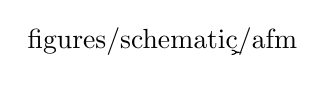
\begin{tikzpicture}[remember picture]
        \node[anchor=south west,inner sep=0] (image) at (0,0) {
          \asyinclude{figures/schematic/afm}};
        \begin{scope}[x={(image.south east)},y={(image.north west)}]
          \draw [decorate,decoration={brace,raise=4pt,mirror}]
              (0.715,0.05) -- (0.715,0.2)
              node [midway,xshift=3pt] (afm-piezo-brace) {};
        \end{scope}
      \end{tikzpicture}
    }
    \hspace{.25in}%
    \subfloat[][]{\label{fig:piezo-schematic}
      \begin{tikzpicture}[remember picture]
        \node[anchor=south west,inner sep=0] (image) at (0,0) {
          \asyinclude{figures/schematic/piezo}};
        \begin{scope}[x={(image.south east)},y={(image.north west)}]
          \draw [decorate,decoration={brace,raise=4pt}]
              (0,0.1) -- (0,0.9)
              node [midway,xshift=-3pt] (piezo-brace) {};
          \draw [overlay,out=0,in=180] (afm-piezo-brace) to (piezo-brace);
        \end{scope}
      \end{tikzpicture}
    }
    \caption{\protect\subref{fig:afm-schematic} Operating principle
      for an Atomic Force Microscope\index{AFM}.  A sharp tip
      integrated at the end of a cantilever interacts with the sample.
      Cantilever bending is measured by a laser reflected off the
      cantilever and incident on a position sensitive photodetector.
      \protect\subref{fig:piezo-schematic} Schematic of a tubular
      piezoelectric actuator.  In our AFM, the substrate is mounted on
      the top end of the tube, and the bottom end is fixed to the
      microscope body.  This allows the piezo to control the relative
      position between the substrate and the AFM cantilever.  The
      electrodes are placed so radial electric fields can be easily
      generated.  These radial fields will cause the piezo to expand
      or contract axially.  The $z$ voltage causes the tube to expand
      and contract uniformly in the axial direction.  The $x$ and $y$
      voltages cause expansion on one side of the tube, and
      contraction (because of the reversed polarity) on the other side
      of the tube.  This tilts the tube, shifting the sample
      horizontally.\label{fig:afm-schematic-and-piezo}}
  \end{center}
\end{figure}

% really, AFM can do this ;)
The forces that can be applied and measured with an AFM range from
tens of piconewtons to hundreds of nanonewtons.  The investigation of
the unfolding and refolding processes of individual protein molecules
by the AFM is feasible because many globular proteins unfold under
external forces in this range.  Since elucidating the mechanism of
protein folding is currently one of the most important problems in
biological sciences, the potential of the AFM for revealing
significant and unique information about protein folding has
stimulated much effort in both experimental and theoretical research.

\section{Protein polymer synthesis---Titin I27}
\label{sec:polymer-synthesis}

Early experiments in force spectroscopy involved
DNA\citep{bustamante94,florin95}, but before long they were also
investigating proteins.  Native titin was one of the first proteins
studied with force spectroscopy\index{titin}\citep{rief97a}.  Titin is
a muscle protein involved in passive elasticity
(\cref{fig:skeletal-muscle}), so it is an ideal subject when examining
the effect of mechanical force\citep{labeit95}.  Titin is also
interesting because, while it is one of the largest known proteins, it
is composed of a series of globular domains.  When \citet{rief97a}
carried out their seminal unfolding experiment, they observed a very
characteristic sawtooth as the domains unfolded (see
\cref{sec:procedure} for a discussion of these sawteeth).

\begin{figure}
  \includegraphics[width=0.7\textwidth]{figures/binary/skeletal_muscle}%
  \caption{Biological role of titin\index{titin}.  Moving clockwise
    from the upper left you can see a bone/muscle group, a muscle
    fiber, a myofibril, and a sarcomere.  In the sarcomere, the white,
    knobbly filaments are actin.  The myosin bundles are blue, and the
    titin linkers are red.  When the muscle contracts, the myosin
    heads walk up the actin filiaments, shortening the sarcomere.
    When the muscle relaxes, the myosin heads release the actin
    filimants and slide back, lengthening the sarcomere.  Titin
    functions as an entropic spring that keeps the myosin from falling
    out of place during the passive, relaxed stage.  This figure is
    adapted from \citet{skeletal_muscle}.\label{fig:skeletal-muscle}}
\end{figure}

Unfortunately, it is difficult to analyze the unfolding of native
titin, because the heterogenous globular domains make it hard to
attribute a particular subdomain to a partuclar unfolding event.
Unfolding a single domain is not feasable because the large radius of
curvature of an AFM tip ($\sim20\U{nm}$\citep{olympus-tr400psa})
dwarfs the radius of a globular domain
($\sim2\U{nm}$\citep{improta96}).  When such a large tip is so close
to the substrate, van der Waals forces and non-specific binding with
the surface dominate the tip-surface interaction.  In order to
increase the tip-surface distance while preserving single molecule
analysis, \citet{carrion-vazquez99b} synthesized a protein composed of
eight repeats of immunoglobulin-like domain 27 (I27\index{I27}), one
of the globular domains from native titin (\cref{fig:I27}).  Octameric
I27 produced using their procedure is now available
commercially\citep{athenaes-i27o}.
%
\nomenclature[text ]{I27}{Immunoglobulin-like domain 27 from human
  titin.}

\begin{figure}
  \includegraphics[width=2in]{figures/i27/1TIT}
  \caption{I27, the immunoglobulin-like domain 27 from human titin
    (\href{http://dx.doi.org/10.2210/pdb1tit/pdb}{PDB ID: 1TIT})%
    \citep{improta96}.  The entire domain is $4.7\U{nm}$ from end to
    end.  Figure generated with \citetalias{pymol}.
    \label{fig:I27}\index{I27}}
\end{figure}

Synthetic proteins are generally produced by creating a plasmid coding
for the target protein, inserting the plasmid in a bacteria, waiting
while the bacteria produce your protein, and then purifying your
proteins from the resulting culture.  In this case,
\citet{carrion-vazquez99b} extracted messenger RNA coding for titin
from human cardiac tissue\citep{rief97a}, and used reverse
transcriptase to generate a complementary DNA (cDNA) library from
human cardiac muscle messenger RNA.  This cDNA is then amplified using
the polymerase chain reaction (PCR), with special primers that allow
you to splice the resulting cDNA into a plasmid (which ends up with
one I27).  Then they ran another PCR on the plasmid, linearized the
plasmid with two restriction enzymes, and grafted two I27-containing
sections together to form a new plasmid (now with two I27s,
\cref{fig:plasmid}).  Another PCR-split-join cycle produced a plasmid
with four I27s, and a final cycle produced a plasmid with eight.  The
eventual plasmid vector has the eight I27s and a host-specific
promoter that causes the bacteria to produce large quantities of I27.
The exact structure of the generated octamer
is\citep{carrion-vazquez99b}
\nomenclature[text ]{cDNA}{Complementary DNA.}
\nomenclature[text ]{PCR}{Polymerase chain reaction.}

\begin{center}
  Met-Arg-Gly-Ser-(His)$_6$-Gly-Ser-(I27-Arg-Ser)$_7$-I27-\ldots-Cys-Cys
  \label{eq:I27}
\end{center}

\begin{figure}
  \includegraphics[width=0.9\textwidth]{figures/binary/kempe85-fig2}%
  \caption{Example of gene duplication via plasmid splicing
    (\xref{kempe85}{figure}{2}).  \citet{kempe85} use a different
    gene, but some of the restriction enzymes are shared with
    \citet{carrion-vazquez99b}.  The overall approach is
    identical.\label{fig:plasmid}}
\end{figure}

\index{\species{Escherichia coli}}
The plasmid is then transformed into the host, usually
\species{Escherichia coli}\citep{carrion-vazquez99b,bartels03,ma10} or
a proprietary equivalent such as Agilent's SURE 2 Supercompetent
Cells\citep{agilent-sure2,carrion-vazquez00}.  The infected cells are
cultured to express the protein.
%
\nomenclature[text ]{Bacterial transformation}{The process by which
  bacterial cells take up exogenous DNA molecules.}
\nomenclature[text ]{Exogenous DNA}{DNA that is outside of a cell.}

The octamer is then purified from the culture using immobilized metal
ion affinity chromatography (IMAC), where the His-tagged end of the
octamer covalently bonds to a metal ion that is bound to the column
media (e.g. Ni-NTA\index{Ni-NTA} coated
beads)\citep{carrion-vazquez00,bartels03,ma10}.  Once the rest of the
broth has been washed out of the chromatography column, the octamer is
eluted via either another molecule which competes for the metal
ions\citep{ma10} or by changing the pH so the octamer is less
attracted to the metal ion.
%
\nomenclature[text ]{IMAC}{Immobilized metal ion affinity
  chromatography.}
\nomenclature[text ]{Ni-NTA}{Nickle nitrilotriacetic acid.}

\nomenclature[text ]{Ala}{Alanine, an amino acid.}
\nomenclature[text ]{Arg}{Arginine, an amino acid.}
\nomenclature[text ]{Asn}{Asparagine, an amino acid.}
\nomenclature[text ]{Asp}{Aspartic acid, an amino acid.}
\nomenclature[text ]{Cys}{Cystine, an amino acid.}
\nomenclature[text ]{Glu}{Glutamic acid, an amino acid.}
\nomenclature[text ]{Gln}{Glutamine, an amino acid.}
\nomenclature[text ]{Gly}{Glycine, an amino acid.}
\nomenclature[text ]{His}{Histidine, an amino acid.}
\nomenclature[text ]{Ile}{Isoleucine, an amino acid.}
\nomenclature[text ]{Leu}{Leucine, an amino acid.}
\nomenclature[text ]{Lys}{Lysine, an amino acid.}
\nomenclature[text ]{Met}{Methionine, an amino acid.}
\nomenclature[text ]{Phe}{Phenylalanine, an amino acid.}
\nomenclature[text ]{Pro}{Proline, an amino acid.}
\nomenclature[text ]{Ser}{Serine, an amino acid.}
\nomenclature[text ]{Thr}{Threonine, an amino acid.}
\nomenclature[text ]{Trp}{Tryptophan, an amino acid.}
\nomenclature[text ]{Tyr}{Tyrosine, an amino acid.}
\nomenclature[text ]{Val}{Valine, an amino acid.}

\section{Sample preparation}
\label{sec:sample-preparation}

In mechanical unfolding experiments, one end of the protein is bound
to a substrate and the other binds to the AFM tip.  This allows you to
stretch the protein by increasing the tip-substrate distance using the
piezo.  A common approach is to synthesize proteins with cystine
residues on one end (\cref{eq:I27}) and allow the cystines to bind to
a gold surface\citep{carrion-vazquez99b,carrion-vazquez00,ulman96}.

We prepare gold-surfaces by sputtering gold onto freshly cleaved mica
sheets in a vacuum.  The mica keeps the gold surface protected from
contamination until it is needed.  In order to mount the gold on our
AFM, we glue glass coverslips to the gold using a two part epoxy. %(TODO)
Instead of using mica to protect the gold surface, some labs
evaporate the gold directly onto the coverslips immediately before
running an experiment\citep{carrion-vazquez99b}.

When it is time to deposit proteins on the surface, we peel a
coverslip off the gold-coated mica, exposing the gold surface that had
previously been attached to the mica.  We dispense $5\U{$\mu$L}$ of
I27 solution ($65\U{g/$\mu$L}$) on the freshly-exposed gold, followed
by $5\U{$\mu$L}$ of phosphate buffered saline (PBS).  We allow the
protein to bind to the gold surface for 30 mintues and then load the
coated coverslips into our AFM fluid cell. There are a number of
similar PBS recipes in common
use\citep{florin95,carrion-vazquez00,lo01,brockwell02}, but our PBS is
diluted from 10x PBS stock composed of $1260\U{mM}$ NaCl, $72\U{mM}$
\diNaHPO, and $30\U{mM}$ \NadiHPO\citep{chyan04}.
%
\index{Phosphate buffered saline (PBS)}
\nomenclature[text ]{PBS}{Phosphate buffered saline.}

As an alternative to binding proteins to gold, others have used
EGTA\citep{kellermayer03},
Ni-NTA\citep{schmidt02,itoh04,sakaki05,berkemeier11}, or silanized
glass\citep{sundberg03,ma10}.  Some groups have also functionalized
the cantilever tips by coating them with molecules designed to bind to
the protein\citep{lee05}.  Of these, a Ni-NTA coating is the most
popular\citep{schmitt00}.
%
\nomenclature[text ]{EGTA}{Ethylene glycol tetraacetic acid}

\section{Calibcant}
\label{sec:calibcant:procedure}

A calibration run based on \cref{eq:kappa} consists of bumping the
surface with the cantilever tip to measure $\sigma_p$, measuring the
buffer temperature $T$ with a thermocouple, and measuring thermal
vibration when the tip is far from the surface to extract the fit
parameters $G_{1f}$, $f_0$, and $\beta_f$.  I've written the
\calibcant\ package to carry out this calibration procedure, building
on packages in the \pyafm\ stack (\cref{fig:calibcant:stack}).

\begin{figure}
  \tikzstack{black!20}{}
  \caption{Dependency graph for \calibcant, which shares the
    \pyafm\ stack with \unfoldprotein (\cref{fig:pyafm:stack}).  The
    only difference is that the ``brain'' module controlling the stack
    has changed from \unfoldprotein\ to
    \calibcant.\label{fig:calibcant:stack}}
\end{figure}

\subsection{Photodiode calibration}
\label{sec:calibcant:bump}

To calculate the photodiode sensitivity $\sigma_p$, we need surface
bumps with a clearly delimited contact slope.  The \calibcant\ package
uses \imint{python}|AFM.move_just_onto_surface|
(\cref{sec:pyafm:pyafm}) to position the cantilever tip a configurable
distance off the surface (\cref{sec:pyafm:h5config}).  Then
\calibcant\ uses the \pypiezo\ component (\cref{sec:pyafm:pypiezo}) to
ramp the tip towards the surface a configurable distance before
returning the tip to its original position.  The cantilever deflection
during this approach--retract cycle is analyzed to measure $\sigma_p$
(\cref{fig:calibcant:bump}).

\begin{figure}
  \begin{center}
    \includegraphics[width=0.8\textwidth]{figures/calibcant/bump}
    \caption{Measuring the photodiode sensitivity $\sigma_p$ by
      bumping the cantilever tip on the substrate surface.  In the
      first panel, the blue dots are experimental data, the green line
      is the heuristic guess at initial fitting parameters, and the
      red line is the optimized fit.  The second panel shows the
      residual (measured data minus modeled data) for the bump.  In
      both panels, there are two deflection measurements at each
      position, one taken during the approach phase and another taken
      during the retraction phase.  This is the first bump from the
      2013-02-07T08-20-46 calibration.\label{fig:calibcant:bump}}
  \end{center}
\end{figure}

The retraction data is analyzed using a similar approach to \pypiezo's
surface detection algorithm to extract the slope of the contact
region.  Where \pypiezo\ uses a bilinear model
(\cref{eq:bilinear-surface}), \calibcant\ uses a limited linear model:

\begin{equation}
  d(z) = \begin{cases}
      d_\text{rail}  &  z \le z_\text{rail} \\
      d_\text{kink} + \sigma_p (z - z_\text{kink})
        &  z_\text{rail} \le z \le z_\text{kink} \\
      d_\text{kink}  &  z \ge z_\text{kink}
    \end{cases}
  \label{eq:limited-linear-surface}
\end{equation}

The fitted parameters are the surface contact point $(z_\text{kink},
d_\text{kink})$ and the contact slope $\sigma_p$.  ADCs can only
digitize voltages between the rails of their power supply, and the
clipping deflection $d_\text{rail}$ is the deflection ADC's maximum
measureable voltage ($2^{16}\U{bits}$ for our 16-bit ADCs).

By explicitly modeling the clipping deflection, we avoid the need for
manual intervention when the configured approach distance is too large
for the cantilever geometry and a bump pushes too hard.  With short
cantilevers, even small tip deflection distances can generate large
laser deflection angles (\cref{fig:afm-schematic}), leading to
unmeasurable deflection voltages.  One of the unfolding pulls in
\cref{fig:pyafm:labview-comparison:many} exhibits this effect,
although it was recorded using a different stack.

An alternative approach using sinusoidal piezo oscillation in the
contact region has been proposed by \citet{materassi09}, on the
grounds that it is more reliable and easily automated than an explicit
bump and manual analysis.  While I agree that \emph{any} automated
method is likely better than manual analysis, I feel that the
difference between using an automated bump with a linear contact fit
and using an automated oscillation with a linear contact fit is likely
negligible.

\subsection{Temperature measurements}
\label{sec:calibcant:temperature}

After a series of surface bumps have been made to measure $\sigma_p$,
the stepper motor is used to move the cantilever a configurable
distance from the surface (generally $\sim30\U{$\mu$m}$).  While the
cantilever settles down after the jarring stepper motion, we measure
the buffer temperature using \pypid\ (\cref{sec:pyafm:pypid}), a
Melcor Series MTCA Thermoelectric Cooler Controller\citep{melcor}, and
a type E thermocouple\footnote{Part number 5TC-TT-E-30-72 from OMEGA
  Engineering Inc.\citep{omega}.  Breaking down the product number,
  it's a five pack of thermocouples (5TC) with perfluoroalkoxy
  insulation (TT), type E metals (chromel--constantan), number 30 AWG
  wires ($0.255\U{mm}$ diameter), in a $72\U{inch}$ length.}.  The
thermocouple is inserted through one of the ports in the AFM fluid
cell, so the thermocouple tip is in the buffer less than $3\U{mm}$
from the cantilever tip.% TODO: measure distance

\Cref{eq:kappa} depends on the \emph{absolute} temperature, so labs
without easy access to a thermocouple can probably get away with
estimating the buffer temperature.  Errors of $5\U{K}$ from an actual
temperature of around $300\U{K}$ will be within 1.7\% of the actual
value.  The effect of this error on $\kappa$ will be modest, but see
\cref{sec:calibcant:discussion:errors} for a full discussion.

\subsection{Thermal vibration}
\label{sec:calibcant:vibration}

After the temperature measurements are complete, we measure the
cantilever's thermal vibration without moving the piezo
(\cref{fig:calibcant:vibration}).  The parameters controlling these
vibrations are configurable (with \hFconfig,
\cref{sec:pyafm:h5config}), but the default values are:

\begin{description}
  \item[frequency] The sampling frequency, which defaults to
    $50\U{kHz}$.  This value gives a Nyquist frequency of $25\U{kHz}$,
    which is well above our resonant cantilever frequencies
    ($\sim5\U{kHz}$ in the buffer).
  \item[sample time] The acquisition time in seconds.  This is rounded
    up as required so the number of samples will be an integer power
    of two for efficient Fourier transformation.  It defaults to
    $1\U{s}$.
  \item[model] The vibration model.  This selects the fitting method
    for extracting the variance $\avg{V_p(t)^2}$.  By default,
    \cref{eq:psd-Vp} is used, but you can add the constant offset
    (discussed below) or use the na\"{\i}ve
    $\avg{V_p(t)^2}=\sum(V_p^2)/N$.
  \item[minimum fit frequency] The low-frequency end of the
    \PSD\ usually has a good deal of noise due to detector drift or
    background (non-cantilever) vibrations.  This parameter allows
    you to select a window of the \PSD\ for fitting that excludes the
    troublesome low-frequency region.  It defaults to $500\U{Hz}$.
  \item[maximum fit frequency] For completeness, you can also set a
    high-frequency cutoff, although I've never had to use this
    parameter.
  \item[chunk-size, overlap, \ldots] Assorted parameters for Fourier
    transforms used to compute the \PSD.
\end{description}

\begin{figure}
  \begin{center}
    \subfloat[][]{\label{fig:calibcant:vibration:offset}
      \includegraphics[width=0.8\textwidth]{figures/calibcant/vibration}}
    \caption{\protect\subref{fig:calibcant:vibration:offset}Measuring
      the cantilever's thermal vibration.  The top panel shows the raw
      time series data in bins, the middle panel shows the
      distribution of bin values with a Gaussian fit, and the bottom
      panel shows the $\PSD_f(V_p,f)$ with a fit following
      \cref{eq:psd-Vp-offset}.  The constant offset $P_{0f}$, drawn as
      the horizontal line in the third panel, accounts for white noise
      in the measurement circuit\citep{burnham03}.  The vertical line
      marks the peak frequency $f_\text{max}$
      (\cref{eq:peak-frequency}).  Only data in the blue region was
      used when computing the best fit.  This is the first vibration
      from the 2013-02-07T08-20-46 calibration, yielding a fitted
      variance $\avg{V_p(t)^2}=96.90\pm0.99\U{mV$^2$}$.  The narrow
      spike around $14.3\U{kHz}$ is not due to the cantilever's
      thermal vibration, and rejecting noise like this is the reason
      we use a frequency-space fit to calculate the thermal deflection
      variance.
      \label{fig:calibcant:vibration}}
  \end{center}
\end{figure}

\begin{figure}
  \ContinuedFloat
  \begin{center}
    \subfloat[][]{\label{fig:calibcant:vibration:no-offset}
      \includegraphics[width=0.8\textwidth]{figures/calibcant/vibration-no-offset}}
    \caption{\protect\subref{fig:calibcant:vibration:no-offset}This is
      the same data as in
      \protect\subref{fig:calibcant:vibration:offset} fit with
      \cref{eq:psd-Vp}, yielding a fitted variance
      $\avg{V_p(t)^2}=120.92\pm0.90\U{mV$^2$}$.  The third panel is
      very similar to figure 2 in \citet{florin95}, but they do not go
      into further detail on the method or model.  They may be fitting
      their data to \cref{eq:lorentzian}, see
      \cref{sec:calibcant:lorentzian}.  Another similar figure is in
      \citet{hutter93}.}
  \end{center}
\end{figure}

\Cref{eq:psd-Vp} decreases for large frequencies, but the measured
\PSD\ levels out (\cref{fig:calibcant:vibration:no-offset}).  I
attribute this to background white noise in the measurement circuit,
and not due to cantilever oscillation.  To avoid artificially
inflating the estimated $\avg{V_p(t)^2}$, I created an alternative
model for $\PSD_f(V_p,f)$ that adds a frequency-independent offset
$P_{0f}$\citep{burnham03}.

\begin{equation}
  \PSD_f(V_p, f) = \frac{G_{1f}}{(f_0^2-f^2)^2 + \beta_f^2 f^2} + P_{0f} \;.
  \label{eq:psd-Vp-offset}
\end{equation}

Plots of \cref{eq:psd-Vp-offset} fits look better than
\cref{eq:psd-Vp} fits (\cref{fig:calibcant:vibration}), but the
significance on the variance calculated with
\cref{eq:avg-Vp-Gone-f} depends on the amount of background noise
in the vibration data.  With over an order of magnitude difference
between the power of the damped harmonic oscillator peak and the
background noise, the effect of $P_{0f}$ will be small.  With noisier
setups, removing the white background noise can lead to a significant
difference.  The fitted variance $\avg{V_p(t)^2}$ of my
2013-02-07T08-20-46 data shifts from $120.92\pm0.90\U{mV$^2$}$ using
\cref{eq:psd-Vp} to $96.90\pm0.99\U{mV$^2$}$ using
\cref{eq:psd-Vp-offset}, a 20\% decrease.  The calculated spring
constant increases from $43.3\pm{2.1}$ to $54.1\pm2.7\U{mN/m}$, a 25\%
increase.  Changes of this magnitude are important for accurate
unfolding force calibration.

\section{Cantilever spring constant calibration}
\label{sec:cantilever-calib:intro}

In order to measure forces accurately with an AFM, it is important to
measure the cantilever spring constant $\kappa$\index{$\kappa$}.  The
force exerted on the cantilever can then be deduced from its
deflection via Hooke's law,\index{Hooke's law}
\begin{equation}
  F=-\kappa x \;,  \label{eq:hooke}
\end{equation}
where $x$ is the perpendicular displacement of the cantilever tip
($x_c$ in \cref{fig:unfolding-schematic}).
%
\nomenclature[sr ]{$F$}{Force (newtons).}
\nomenclature[sg k ]{$\kappa$}{Spring constant (newtons per meter).}
\nomenclature[sr ]{$x$}{Displacement (meters).}

The basic idea is to use the equipartition theorem, which gives the
thermal energy per degree of freedom.  For a simple harmonic
oscillator, the only degree of freedom is $x$, so we
have\citep{hutter93}
\begin{equation}
  \frac{1}{2} \kappa \avg{x^2} = \frac{1}{2} k_BT \;, \label{eq:equipart}
\end{equation}
where $k_B$ is Boltzmann's constant, $T$ is the absolute temperature,
and $\avg{x^2}$ is the average value of $x^2$ measured
over a long time interval.
%
\nomenclature[sr ]{$k_B$}{Boltzmann's constant,
  $k_B = 1.380 65\E{-23}\U{J/K}$\citep{codata-boltzmann}.}
\nomenclature[sr ]{$T$}{Absolute temperature (Kelvin).}
\nomenclature[o  ]{$\avg{s(t)}$}{Mean (expectation value) of a
  time-series $s(t)$
  \begin{equation}
    \avg{A} \equiv \iLimT{A} \;.
  \end{equation}}
\nomenclature[o  ]{$\equiv$}{Defined as (\ie\ equivalent to).}

To calculate the spring constant $\kappa$ using \cref{eq:equipart}, we
need to measure the buffer temperature $T$ and the thermal vibration
variance $\avg{x^2}$.  We measure the temperature with a thermocouple
inserted into the AFM fluid cell, and we measure the thermal vibration
by monitoring the cantilever during thermal oscillation when it is far
from the substrate surface.

The raw cantilever deflection data will have sources of noise that are
not due to the cantilever's thermal vibration (e.g.~electronic noise
in the detector).  To avoid biasing $\kappa$, there is a fairly
elaborate theory behind extracting $\avg{x^2}$.  For more detail, see
\cref{sec:calibcant}, where I discuss the $\avg{x^2}$ extraction in
detail and present my open source \calibcant\ tool for automated
cantilever calibration.

